% Optional normalization comparison. Include from the main deck; do not compile alone.
\ifdefined\poreaccessappendixstarted\else\appendix\def\poreaccessappendixstarted{1}\fi
\section[Normalization appendix]{Optional appendix: diffusivity normalization}
\begin{frame}{}
\vfill
{\large\color{tumgray}Optional comparison}\par\vspace{0.4cm}
{\LARGE\color{tumblue}\textbf{The diffusivity-normalized descriptor}}\par\vspace{0.5cm}
{\large Definition, length convention and comparison with direct conductance}
\vfill
\end{frame}
\begin{frame}{Dimensional normalization is an optional descriptor choice}
\begin{columns}[T,onlytextwidth]
\column{0.48\textwidth}\small
\hi{Conductance and diffusivity units}
\[G_{\rm access}=\dot n/\Delta c\quad [\mathrm{m^3/s}]\]
\[D_{\rm access}=G_{\rm access}H/A_{\rm tube}\quad [\mathrm{m^2/s}]\]
For a uniform sample, $G=DA/L$. Multiplication by $L/A$ removes that sample's area-to-length dependence.
\column{0.48\textwidth}\small
\hi{Length is a modelling convention}
\begin{itemize}
\item These comparisons use the full bed height $H$.
\item The steady conductance ends at an interior plane, not the bed top.
\item Dimensional analysis does not select $H$ or establish $D_{\rm access}=D_{\rm eff}$.
\end{itemize}
\end{columns}
\medskip
\result{The main deck uses $G_{\rm access}$ directly; normalization offers no demonstrated advantage in this ensemble.}
\note{The normalization assigns diffusivity units but does not derive the transient effective coefficient. A homogeneous slab motivates G equals D A over L. Our original convention instead uses full bed height for a conductance ending at an interior plane. Choosing that length is a convention requiring validation. Bed height varies across realizations, so normalized and raw inputs are not exactly equivalent. Both still require calibration against the fitted transient diffusivities.}
\end{frame}
\begin{frame}{Alternative: power law using the normalized descriptor}
  \begin{columns}[c,onlytextwidth]
    \column{0.65\textwidth}
    \centering
    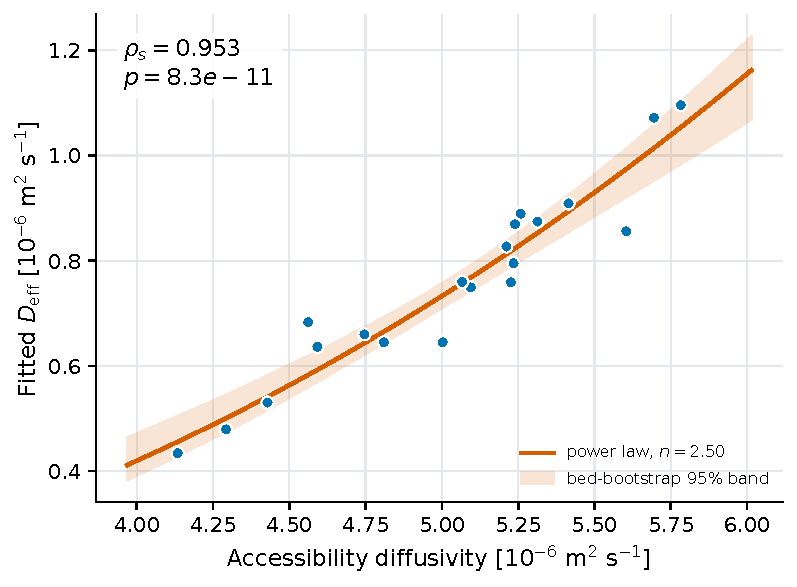
\includegraphics[width=\linewidth,height=0.69\textheight,keepaspectratio]{figures/fig_closure_power_law.pdf}
    \column{0.32\textwidth}
    \small
    \hi{Selected closure}
\[
 \frac{D_{\rm eff}}{D_m}=C\left(\frac{D_{\rm access}}{D_m}\right)^n.
\]
\[
 D_{\rm access}=\frac{G_{\rm access}H}{A_{\rm tube}}.
\]
\medskip
The shaded band shows bootstrap uncertainty in the fitted relationship.
  \end{columns}
  \vspace{0.12cm}
  {\small\result{The fitted exponent is $n\approx2.50$ for this ensemble.}}
\note{Each bed supplies an accessibility diffusivity and a diffusivity fitted to its transient response. D sub m is the fixed molecular diffusivity defined on slide 8. Dividing both diffusivities by D sub m makes C dimensionless. This plot fits all twenty beds; its band is pointwise bootstrap uncertainty in the relationship, not a prediction interval for an individual bed. The power law is positive for positive access and tends to zero with access. We retain it as a physically admissible empirical form, not as an outright predictive winner. The next slide includes both linear-with-intercept alternatives. The exponent is specific to this ensemble.}
\end{frame}

\begin{frame}{Normalized descriptor and raw-conductance linear comparison}
  \begin{columns}[c,onlytextwidth]
    \column{0.62\textwidth}
    \centering
    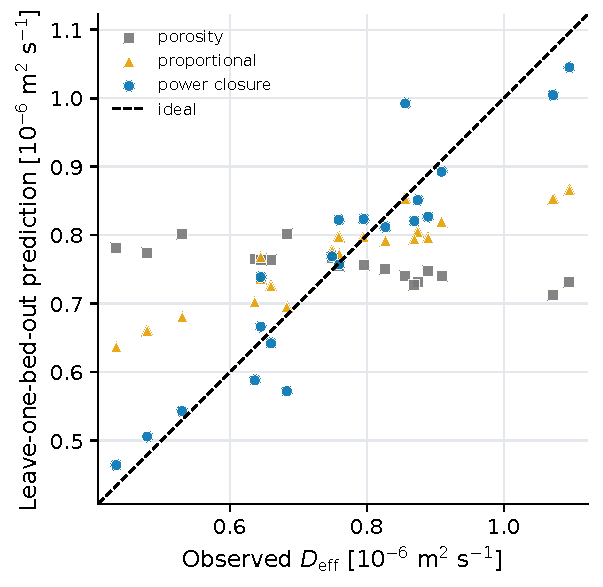
\includegraphics[width=\linewidth,height=0.69\textheight,keepaspectratio]{figures/fig_closure_held_out.pdf}
    \column{0.35\textwidth}\small
    \hi{Forms and held-out $R^2$}
    \begin{tabular}{lr}\toprule
    Predictor / form & $R^2$\\\midrule
    $a_GG_{\rm access}+b_G$ & 0.898\\
    $CD_m(D_{\rm access}/D_m)^n$ & 0.890\\
    $a_DD_{\rm access}+b_D$ & 0.881\\
    $\alpha D_{\rm access}$ & 0.555\\
    $a_0+a_1\varepsilon_b$ & $-0.234$\\\bottomrule
    \end{tabular}
    \medskip\par
    Each expression predicts $D_{\rm eff}$.
    Fit on nineteen beds and predict the omitted bed.
  \end{columns}
  \vspace{0.12cm}
  {\small\result{Power-law and linear-with-intercept scores are close; the power law is not the outright winner.}}
\note{We leave out one entire bed, fit every coefficient on the other nineteen beds, and predict the omitted diffusivity. Repeating this gives twenty predictions per model. The figure now includes the linear model with an intercept using accessibility diffusivity, as in the depth plot, and the separate linear model using raw conductance. Their R squared values are 0.881 and 0.898 respectively, compared with 0.890 for the power law. These are genuinely different predictors because accessibility diffusivity includes the bed height. Small differences in these scores do not establish a clear winner. The power law has positivity and a zero-access limit as modelling advantages. Model and depth selection occurred within this twenty-bed ensemble, so this is internal validation.}
\end{frame}

\begin{frame}{Depth sensitivity of the normalized alternatives}
  \begin{columns}[c,onlytextwidth]
    \column{0.63\textwidth}\centering
    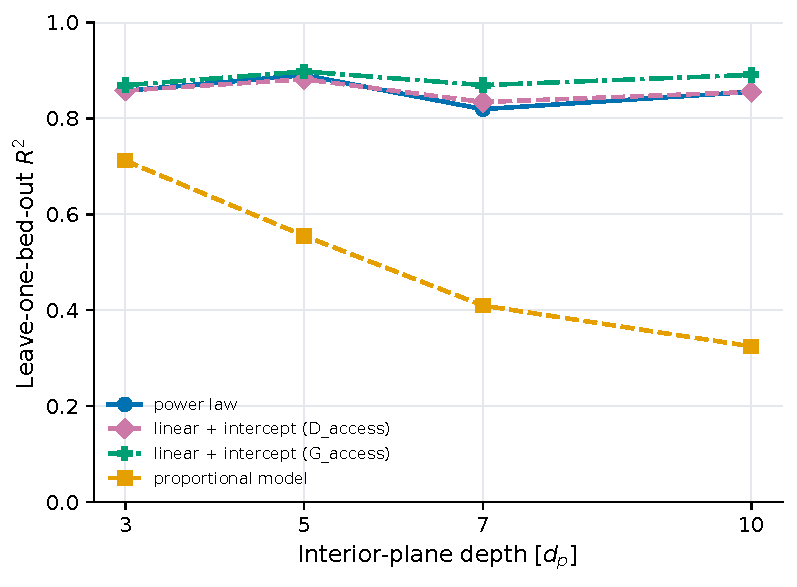
\includegraphics[width=\linewidth,height=0.69\textheight,keepaspectratio]{figures/fig_depth_prediction.pdf}
    \column{0.34\textwidth}\small
    \hi{Four transport models}\par\medskip
    Power law\par
    $D_{\rm eff}=CD_m(D_{\rm access}/D_m)^n$\par\smallskip
    Linear in $D_{\rm access}$ + intercept\par
    $D_{\rm eff}=a_DD_{\rm access}+b_D$\par\smallskip
    Linear in $G_{\rm access}$ + intercept\par
    $D_{\rm eff}=a_GG_{\rm access}+b_G$\par\smallskip
    Proportional\par
    $D_{\rm eff}=\alpha D_{\rm access}$\par\medskip
    Refit on nineteen beds at each depth; predict the omitted bed.
  \end{columns}
  \vspace{0.12cm}
  {\small\result{Power-law $R^2=0.819$--$0.890$ across depths; no consistent advantage over the linear models.}}
\note{All four transport models are now evaluated at every depth with leave-one-bed-out validation, refitting every coefficient using nineteen beds each time. The blue power-law scores at three, five, seven and ten particle diameters are 0.857, 0.890, 0.819 and 0.855. The purple linear-with-intercept model using accessibility diffusivity gives 0.858, 0.881, 0.834 and 0.855. The green linear-with-intercept model using raw conductance gives 0.869, 0.898, 0.869 and 0.891. The orange proportional model gives 0.712, 0.555, 0.409 and 0.324. Both linear forms and the power law remain predictive across these depths, whereas the proportional model deteriorates. The power law is not consistently better than either linear alternative. Five particle diameters gives the highest score for the three flexible forms in this ensemble. The porosity baseline on slide 28 has no inlet-plane depth. Independent beds are needed to assess model and depth selection.}
\end{frame}
